
U okviru sistema je takod1e moguc1e ponishtavnje zahteva od strane Korisnika.

Na slici \ref{fig:dsuponistavanje} se nalazi UML dijagram, dok se na slici \ref{fig:bpmnponistavanje} nalazi BPMN dijagram.


\begin{enumerate}
    \item \textbf{Kratak opis:} Korisnik ponishtava zahtev. Ukoliko je to moguc1e, azhurira se stanje narudzbine. Ako otkazivanje nije moguc1e, korisniku se shalje informacija o neuspelom otkazivanju.
    
    \item \textbf{Uchesnici:} Korisnik, Logistichar
    \item \textbf{Preduslovi:} Korisnik je registrovan u sistemu. Korisnik ima pristup internetu. Sistem je u funkciji. Korisnik je poslao zahtev za transport i ima sachuvanu informaciju o detaljima zahteva uz pomoc1 kojih mozhe pristupiti detaljima zahteva.
    
    \item \textbf{Postuslovi:} U sistemu je pokushaj otkazivanja zabelezhen. Logistichar dobija izveshtaj o otkazivanju i informaciju o trenutnom stanju poshiljke. Korisnik je obaveshten da li je otkazivanje bilo uspeshno ili ne. 
    \item \textbf{Osnovni tok:}
        \begin{enumerate}
            \item[1.1.] Registrovani korisnik pristupa sistemu unoshenjem informacija o svom nalogu.
            
            \item[1.2.] Korisnik pristupa formularu za otkazivanje poshiljke.
            \item[1.3.] U okviru formulara popunjava informacije o ID poshiljke.
            \item[1.4.] Sistem validira unete podatke.
            \item[1.5.] Korisniku se prikazuju informacije o zahtevu.
            \item[1.6.] Korisnik potvrd1uje zahtev za otkazivanje poshiljke. 
            \item[1.7.] Sistem chuva informacije o zahtevu.
            \item[1.8.] Korisniku se shalje informacije o uspeshnosti otkazivanja zahteva.
            \item[1.9.] Logisticharu se shalje izveshtaj o zahtevu za ponishtavanje.
            
        \end{enumerate}
    \item \textbf{Alternativni tokovi:}
            \begin{enumerate}
                \item [A1.] \textbf{Greshka prilikom validacije podataka: }
                Ukoliko u koraku 1.3. korisnik unese pogreshne informacije, sistem obelezhava neispravno polje. 
                Nakon shto korisnik ispravi greshku, proces se nastavlja u koraku 1.3.
                
                \item [A1.] \textbf{Nevalidno otkazivanje: }
                Ukoliko u koraku 1.6. korisnik potvrd1uje otkazivanje zahteva koji je u stanju utovara ili transporta, automatsko otkazivanje nije moguc1e. Zahtev se odbija. Chuvaju se infromacije o zahtevu. Korisnik se obaveshtava o neuspelom otkazivanju.
            \end{enumerate}
        
    \item \textbf{Podtokovi:} /
    \item \textbf{Specijalni zahtevi:} /
    \item \textbf{Dodatne informacije:}/
    
\end{enumerate}



\begin{figure}[h!]
    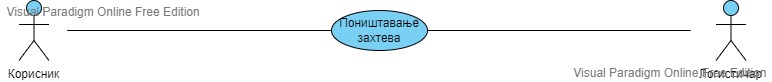
\includegraphics[scale=0.4]{Slike/UML/SUotkazivanjeZahteva.jpg}
    \centering
    \caption{Sluchaj upotrebe: Otkazivanje zahteva za transport}
    \label{fig:dsuponistavanje}
\end{figure}    


\newpage

\begin{figure}[h!]
    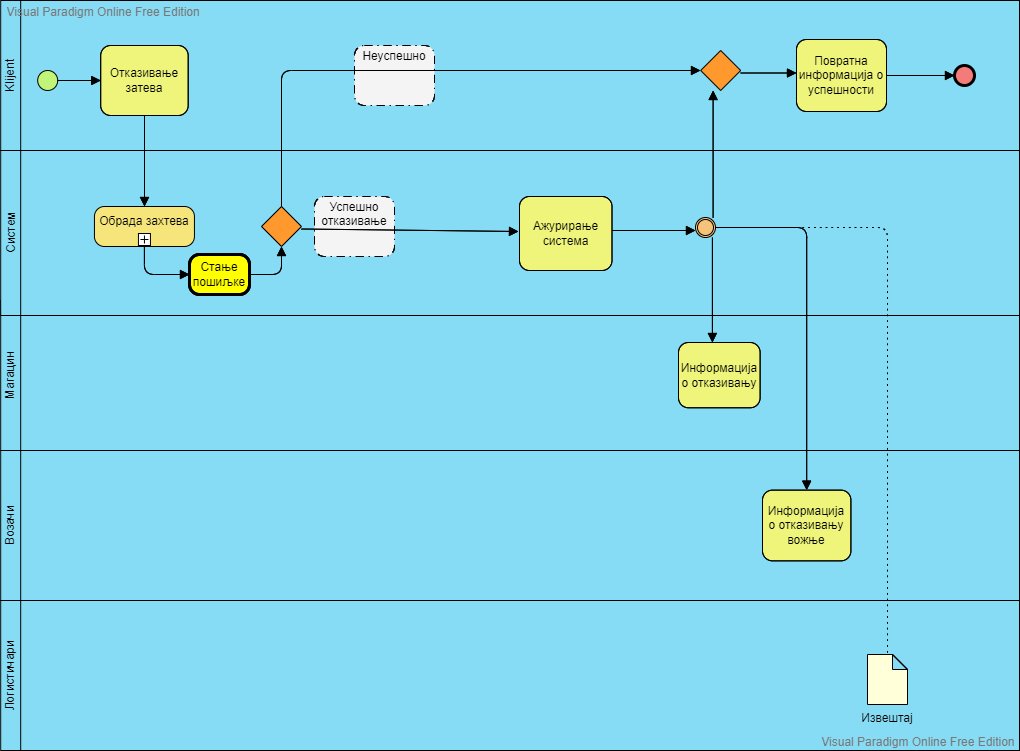
\includegraphics[scale=0.4]{Slike/BPMN/BPMNotkazivanje.png}
    \centering
    \caption{Sluchaj upotrebe: Otkazivanje zahteva za transport}
    \label{fig:bpmnponistavanje}
\end{figure}    



